\documentclass[compress]{beamer}

\usetheme{Szeged}
\usepackage[T1]{fontenc}
\usepackage[utf8]{inputenc}
\usepackage[frenchb]{babel}
%\usepackage[babel=true,kerning=true]{microtype}
\usepackage{tikz,listings,algorithm,algorithmic,hyperref}
\usetikzlibrary{automata,shapes,snakes,arrows}

\tikzstyle{every picture}=[sibling distance=3cm, shorten >=1pt, node distance=2cm,%
	>=stealth', bend angle=10, auto, initial text=]

\title[SEM AU313 - ARD]{AU313 - Application Robotique Dronique}
\author[Charles Lesire]{Charles Lesire-Cabaniols (ONERA / DCSD)\\{\tt charles.lesire@onera.fr}}
\date[2010-2011]{3A-SEM - 2010-2011}

\graphicspath{{../figures/},{../figures/robotics/}}
\lstset{basicstyle=\tiny,tabsize=2,%frame=single,%
	emph={define,domain,requirements,strips,typing,types,predicates,
		action,parameters,precondition,vars,effect,objects,init,goal},%
	emphstyle=\bf}

\begin{document}

\begin{frame}
\titlepage
\end{frame}

\begin{frame}
\tableofcontents[hidesubsections]
\end{frame}

%%% INTRO %%%
\section{Introduction}

\begin{frame}
\tableofcontents[currentsection,hideothersubsections]
\end{frame}

\subsection{Introduction}
\begin{frame}{Définition}
\begin{block}{Robot (étym. : {\it robota} (tchèque), travail, corvée)}
un robot est un système mécanique poly-articulé mû par des actionneurs 
et commandé par un calculateur qui est destiné à effectuer une grande variété de tâches.
\end{block}
\end{frame}

\begin{frame}{Origine}
\begin{columns}
\begin{column}{0.6\linewidth}
	\begin{itemize}
	\item {\it Robot} utilisé pour la première fois en 1921 par Karel Capek dans sa pièce {\it Rossum's Universal Robots} ;
	\item {\it Robotique} émployé pour la première fois par Isaak Asimov en 1941
		\begin{itemize}
		\item {\it I, robot}, 1950
		\item {\it Foundation}, 1951
		\end{itemize}
	\end{itemize}
\end{column}
\begin{column}{.35\linewidth}%
\begin{center}
	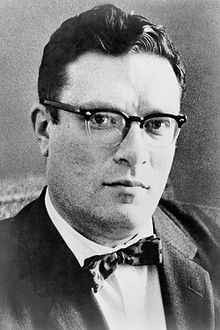
\includegraphics[width=.9\linewidth]{asimov}\\
	\small Isaak Asimov (1965)
\end{center}
\end{column}
\end{columns}
\end{frame}

%%% ROBOTS %%%
\subsection{Robots}
\begin{frame}{Robots manipulateurs}
\begin{itemize}
\item Robots industriels : chaînes de montage, manipulation de produits chimiques, \dots
\item Robots d'assistance médicale
\end{itemize}
\begin{columns}
\column{.45\linewidth}
	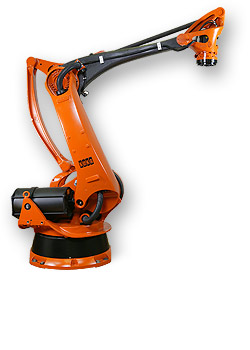
\includegraphics[width=.9\linewidth]{kuka}
\column{.45\linewidth}
	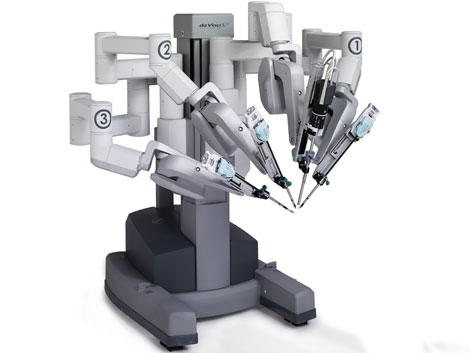
\includegraphics[width=.9\linewidth]{medical}
\end{columns}
\end{frame}

\begin{frame}{Robots d'exploration}
\begin{itemize}
\item Exploration planétaire
\item Exploration d'épaves ou de décombres
\item Déminage, zones radioactives, \dots
\end{itemize}
\begin{columns}
\column{.3\linewidth}
	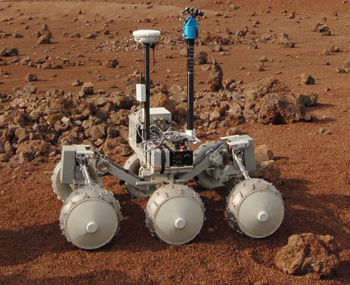
\includegraphics[width=\linewidth]{iares}
\column{.3\linewidth}
	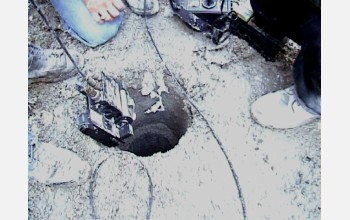
\includegraphics[width=\linewidth]{rescue}
\column{.3\linewidth}
	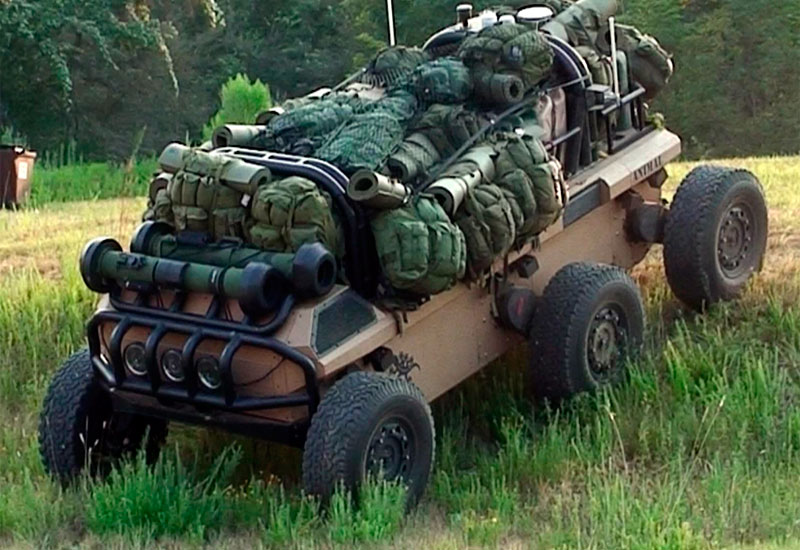
\includegraphics[width=\linewidth]{mule}
\end{columns}
\end{frame}

\begin{frame}{Robots de service}
\begin{itemize}
\item Transport de marchandises
\item Robots ménagers
\item Aide aux personnes
\end{itemize}
\begin{columns}
\column{.3\linewidth}
	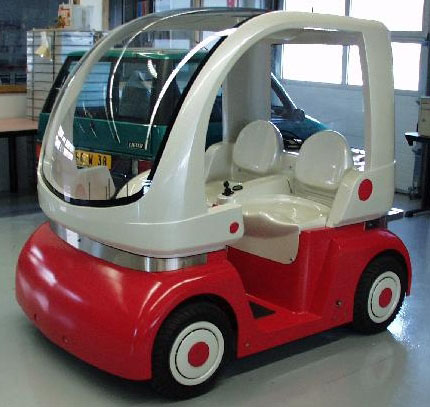
\includegraphics[width=\linewidth]{cycab}
\column{.3\linewidth}
	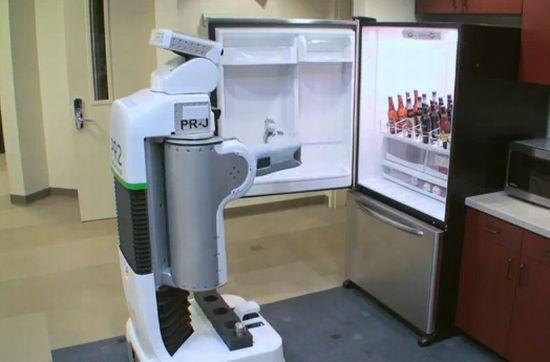
\includegraphics[width=\linewidth]{pr2}
\column{.3\linewidth}
	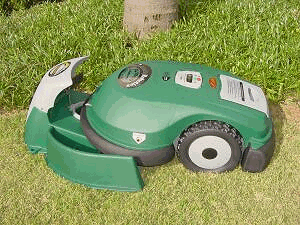
\includegraphics[width=\linewidth]{tondeuse}
\end{columns}
\end{frame}

\begin{frame}{Robots ludiques}
\begin{columns}
\column{.45\linewidth}
	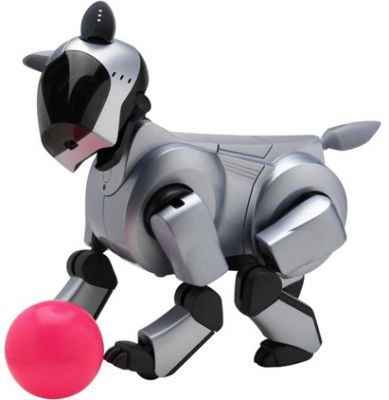
\includegraphics[width=\linewidth]{aibo}
\column{.45\linewidth}
	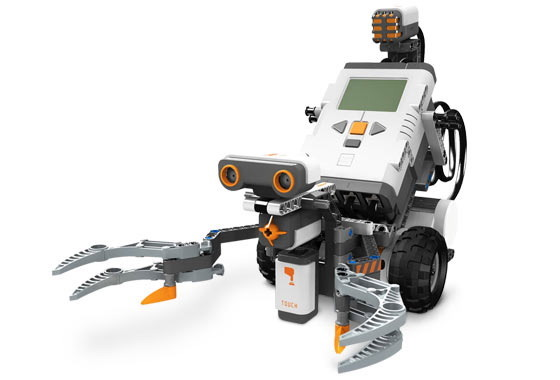
\includegraphics[width=\linewidth]{mindstorm}
\end{columns}
\end{frame}

%%% AUTONOMIE %%%
\subsection{Autonomie}
\begin{frame}{Boucle de décision}
\begin{quote}
Un robot est capable d'extraire de l'information à partir de son environnement et d'utiliser ses connaissances pour décider comment agir. Un robot est équipé de capteurs et d'effecteurs.
\end{quote}
\end{frame}

\begin{frame}{Capteurs / Effecteurs}
\begin{columns}
\column{.45\linewidth}
	Capteurs :
	\begin{itemize}
	\item Caméra
	\item Sonar
	\item Détecteur de lumière
	\item Boussole
	\item GPS
	\item Détecteur de chaleur
	\item \dots
	\end{itemize}
\column{.45\linewidth}
	Effecteurs :
	\begin{itemize}
	\item Roues
	\item Bras
	\item Jambes
	\item Pinces
	\item \dots
	\end{itemize}
\end{columns}
\end{frame}

\begin{frame}{Tâches}
\begin{itemize}
\item Les robots ont un ensemble de tâches à réaliser ;
\item Leur exécution consomme du temps et des ressources ;
\item Des contraintes (temporelles, spatiales, \dots) peuvent leur être associées.
\end{itemize}
\end{frame}

%%%%% ARCHITECTURES %%%%%
\section{Architectures}

\begin{frame}
\tableofcontents[currentsection,hideothersubsections]
\end{frame}

\subsection{Introduction}
\begin{frame}{Programmation}
L'intelligence artificielle d'un robot se résume à un ensemble de programmes écrits sur un ordinateur :
\begin{itemize}
\item les programmes sont écrits dans un langage de programmation ;
\item ils s'exécutent grâce au contrôleur du robot ;
\item ils prennent en entrée les informations obtenues des capteurs et en sortie envoient des ordres aux effecteurs.
\end{itemize}
\end{frame}

\begin{frame}{Programmes}
L'intelligence artificielle d'un robot permet par exemple :
\begin{itemize}
\item l'analyse d'images ;
\item sa localisation et sa navigation ;
\item la gestion des interactions (communications, interfaces) ;
 \item la planification et la prise de décision ;
\item le contrôle de l'exécution des tâches.
\end{itemize}
\end{frame}

%%% SUBSYMBOLIQUE %%%
\subsection{Approche sub-symbolique}

\begin{frame}{Approche sub-symbolique, ascendante ou {\it bottom-up}}
\begin{itemize}
\item 1986, Rodney Brooks : {\it "Elephants don't play chess"}
	\begin{itemize}
	\item L'essentiel pour un robot est d'abord de survivre
	\item Des composants réactifs plutôt que cognitifs
	\item La complexité peut émerger de la somme de comportements simples
	\end{itemize}
\item Vision modeste mais réaliste
	\begin{itemize}
	\item Objectifs modestes : labyrinthes, autonomie énergétique, \dots
	\item Etude de la boucle perception-action
	\item La réactivité et l'adaptation deviennent des enjeux cruciaux
	\end{itemize}
\end{itemize}
\end{frame}

\begin{frame}{Approche traditionnelle}
\begin{center}
\begin{tikzpicture}[node distance=4cm]
	\node (S) {Capteurs};
	\node (B) [right of=S,rotate=90] {\renewcommand{\arraystretch}{1.8}%
		\begin{tabular}{c}
		perception\\\hline
		modélisation\\\hline
		planification\\\hline
		exécution\\\hline
		contrôle
		\end{tabular}};
	\node (A) [right of=B] {Effecteurs};
	\draw (S) edge[->] (B) (B) edge[->] (A);
\end{tikzpicture}
\end{center}
\end{frame}

\begin{frame}{Approche comportementale}
\begin{center}
\begin{tikzpicture}[node distance=4cm]
	\node (S) {Capteurs};
	\node (B) [right of=S] {\renewcommand{\arraystretch}{1.8}%
		\begin{tabular}{c}
		identification de l'objet\\\hline
		construction de la carte\\\hline
		exploration\\\hline
		promenade\\\hline
		évitement  d'obstacle
		\end{tabular}};
	\node (A) [right of=B] {Effecteurs};
	\draw (S) edge[->] (B) (B) edge[->] (A);
\end{tikzpicture}
\end{center}
\end{frame}

\begin{frame}{Approche comportementale}
\begin{center}
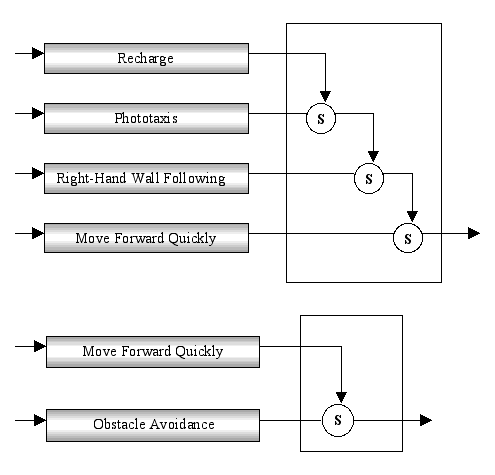
\includegraphics[width=.6\linewidth]{subsomption}
\end{center}
\end{frame}

%%% PAR COUCHES %%%
\subsection{Approche par couches}

\begin{frame}{Architecture LAAS}
\begin{center}
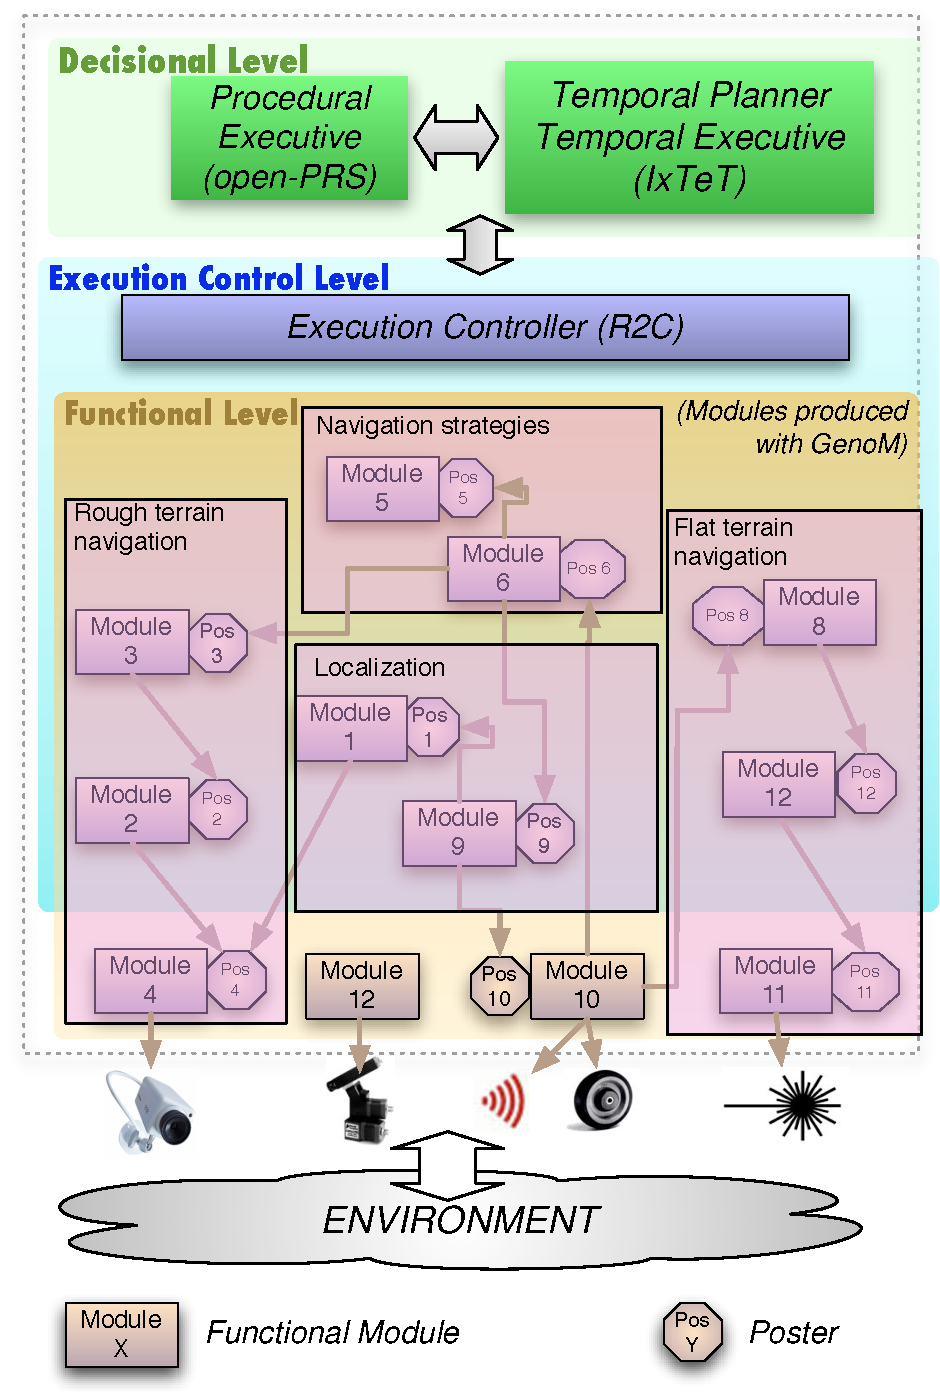
\includegraphics[width=.4\linewidth]{LAAS}
\end{center}
\end{frame}

\begin{frame}{Architecture Claraty (NASA)}
\begin{center}
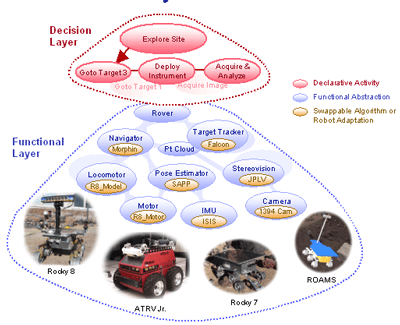
\includegraphics[width=.7\linewidth]{claraty}
\end{center}
\end{frame}

\begin{frame}{Architecture T-REx (MBARI)}
\begin{center}
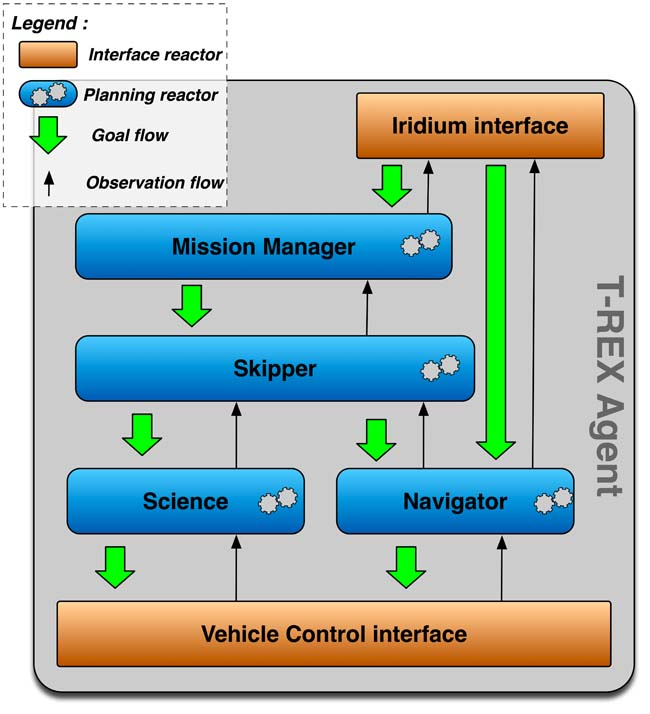
\includegraphics[width=.5\linewidth]{TREX}
\end{center}
\end{frame}

\begin{frame}{Architecture ProCoSA (Onera)}
\begin{center}
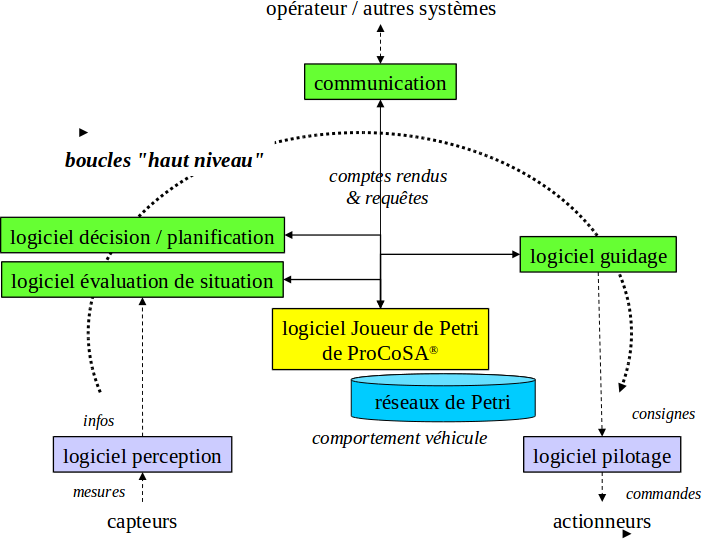
\includegraphics[width=.7\linewidth]{procosa}
\end{center}
\end{frame}

%%% PAR COMPOSANTS %%%
\subsection{Approche par composants}
\begin{frame}{Architecture BIP (LAAS/VeriMAG)}
\begin{center}
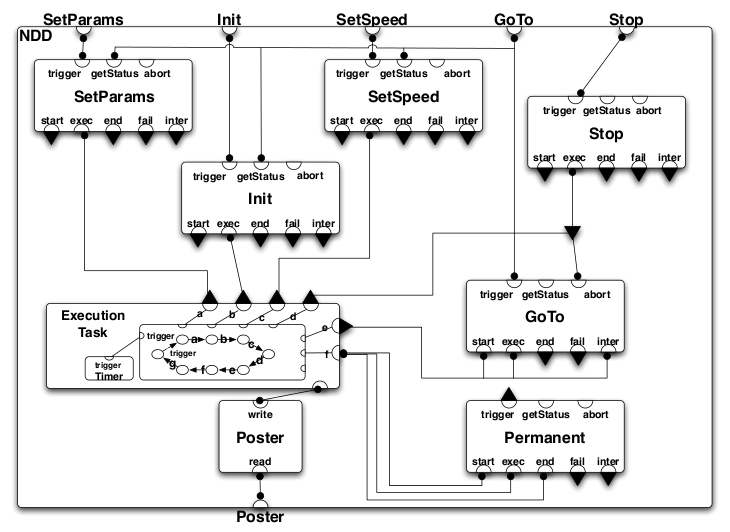
\includegraphics[width=.7\linewidth]{bip}
\end{center}
\end{frame}
\begin{frame}{Architecture Orocos (Univ. Leuven, Onera, NASA, \dots)}
\begin{center}
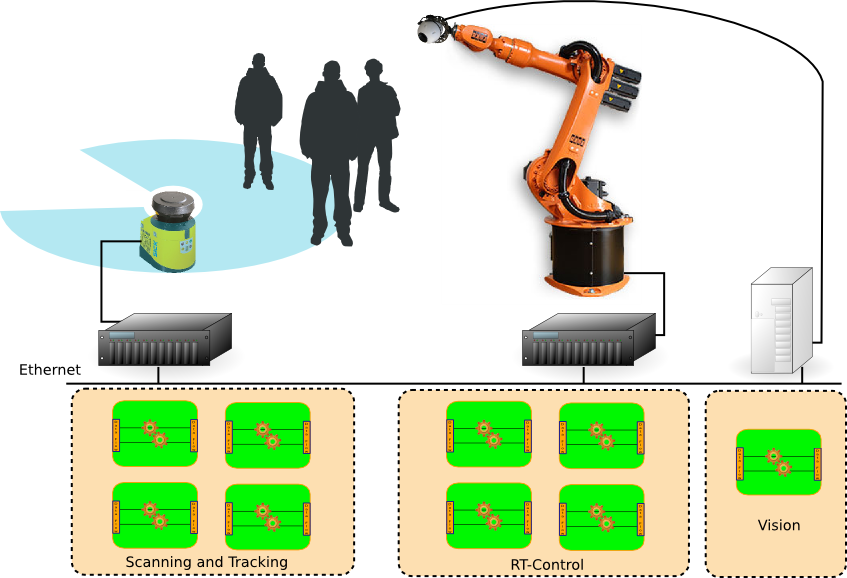
\includegraphics[width=.8\linewidth]{orocos}
\end{center}
\end{frame}

%%% BE %%%
\section{BE}

\begin{frame}
\tableofcontents[currentsection,hideothersubsections]
\end{frame}

\subsection{Sujet}
\begin{frame}{Sujet du BE}
\begin{columns}
\column{.5\linewidth}
	\begin{itemize}
	\item Mission d'exploration de zones, et d'extinction d'incendies
		\begin{itemize}
		\item navigation
		\item exploration
		\item analyse d'images
		\item prise de décision, planification
		\end{itemize}
	\end{itemize}
\column{.45\linewidth}
	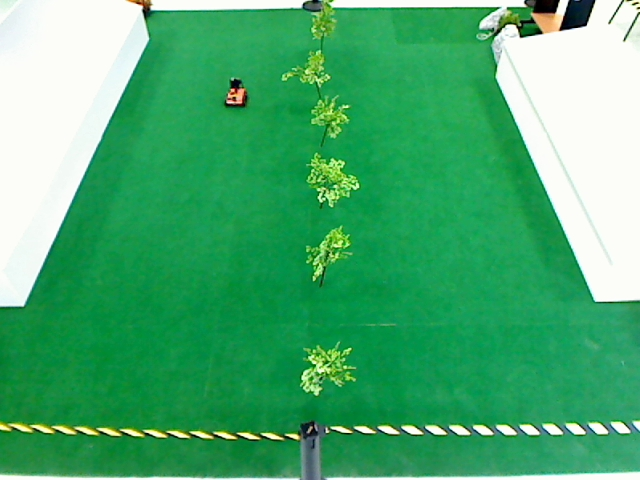
\includegraphics[width=.9\linewidth]{be}
\end{columns}
\end{frame}

\begin{frame}{Sujet du BE}
\begin{itemize}
\item Développement de composants robotiques
	\begin{itemize}
	\item Analyse d'images simplifiée
	\item Sous l'environnement Orocos
	\end{itemize}
\item Déploiement d'une architecture robotique
	\begin{itemize}	
	\item Navigation, Prise d'images, Analyse d'images
	\end{itemize}
\item Supervision de mission
\end{itemize}
\end{frame}

%%% OROCOS %%%
\section{Orocos\hspace{2cm}}

\begin{frame}
\tableofcontents[currentsection,hideothersubsections]
\end{frame}

\subsection{Orocos}
\begin{frame}{Orocos}
Une librairie en C++ qui permet :
\begin{itemize}
\item de créer des composants exécutables, distribuables ;
\item de spécifier des communications temps-réel et "thread-safe" entre composants ;
\item de charger et d'exécuter des scripts (programmes / machines à état) en temps-réel ;
\item d'accéder aux différents attributs des composants et des communications.
\end{itemize}
\end{frame}

\subsection{Composants}
\begin{frame}{Interface d'un composant}
\begin{center}
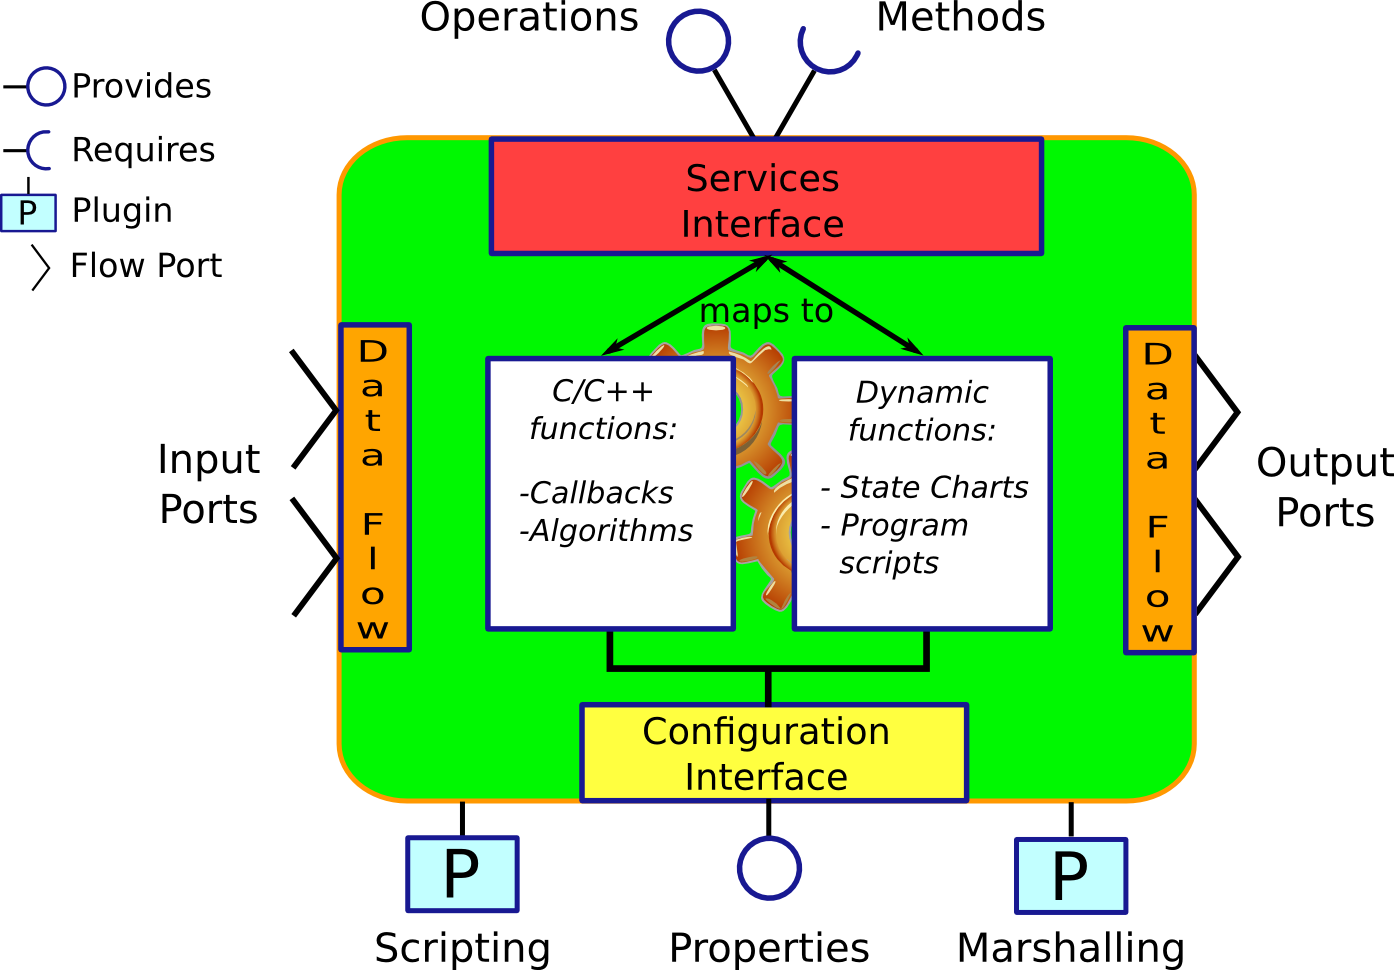
\includegraphics[width=.8\linewidth]{ATaskContext}
\end{center}
\end{frame}

\begin{frame}{Etats d'un composant}
\begin{center}
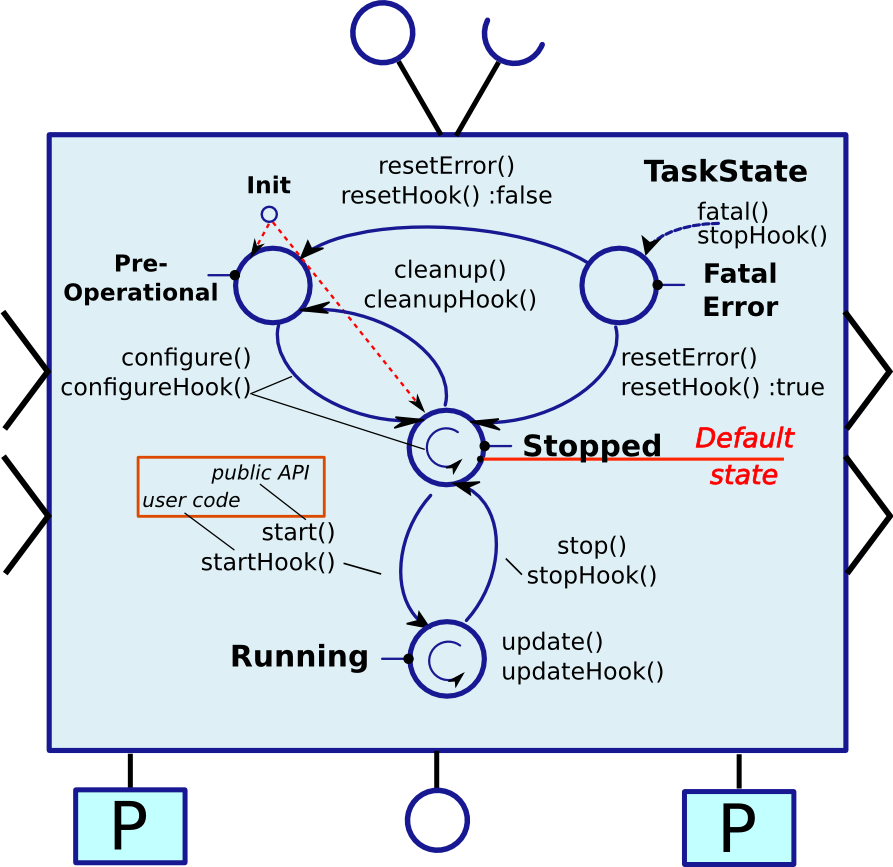
\includegraphics[width=.5\linewidth]{ComponentStatesExtended}
\end{center}
\end{frame}

\begin{frame}[containsverbatim]{Code}
\lstset{language=C++,basicstyle=\tiny,tabsize=3}
\begin{lstlisting}[frame=trBL]
class Mapping : public RTT::TaskContext, MappingAlg {
	MatchingParameters pMatch;
	RTT::Property<std::string> CalibrationFile;
	RTT::Property<std::vector<double> > MapFrame;
	RTT::ReadDataPort<image_t> image_port;
	RTT::ReadDataPort<Vector> position_port;
	RTT::ReadDataPort<Vector> attitude_port;
	RTT::WriteDataPort<std::vector<int> > obstacles;
	RTT::WriteDataPort<image_t> map_port;
	RTT::Command<bool(void)> build_command;
\end{lstlisting}
\end{frame}

\begin{frame}[containsverbatim]{Code}
\lstset{language=C++,basicstyle=\tiny,tabsize=3}
\begin{lstlisting}[frame=trBL]
	Mapping(const std::string& name) :
		RTT::TaskContext(name, PreOperational),
		CalibrationFile("CalibrationFile", "/comment/", ""),
		MapFrame("MapFrame", "/comment/", vector<double>(5,0)),
		position_port("Position"),
		attitude_port("Attitude"),
		image_port("Image"),
		map_port("MapImage"),
		obstacles("MapCounter"),
		build_command("build", &Mapping::build, this)
	{
		ports()->addEventPort(&image_port);
		ports()->addPort(&position_port);
		ports()->addPort(&attitude_port);
		ports()->addPort(&obstacles);
		ports()->addPort(&map_port);
		properties()->addProperty(&pMatch);
		properties()->addProperty(&CalibrationFile);
		properties()->addProperty(&MapFrame);
		commands()->addCommand(&build_command, "Build map."); 
	};
\end{lstlisting}
\end{frame}

\begin{frame}[containsverbatim]{Code}
\lstset{language=C++,basicstyle=\tiny,tabsize=3}
\begin{lstlisting}[frame=trBL]
	virtual bool startHook() {
		// EVA properties
		pMatch.fill(pObsDetect);
		// Init EVA parameters
		initParameters(calibration);
		if (log().getLogLevel() >= Logger::Info)
			dtim_Camera_showIntrinsicParam(&pIntrin);
		// Init Map
		eva_cartoInitialisation(origin_north, ..., &map);
		return true;
	};
	
	virtual void stopHook() {
		if (!flag1st) freeEVA();
		flag1st = true;
	};
\end{lstlisting}
\end{frame}

\begin{frame}[containsverbatim]{Code}
\lstset{language=C++,basicstyle=\tiny,tabsize=3}
\begin{lstlisting}[frame=trBL]
	virtual void updateHook() {
		img = image_port.Get();
		if (!img) {
			log(Error) << "Input image is empty!" << endl;
			return;
		}
		Vector v = position_port.Get();
		Vector w = attitude_port.Get();
		setExtrinsicParameters(v, w);
		if (flag1st) {
			flag1st = false;
			createEVA();
			return;
		}
		// Detection
		double pct = detect();
		log() << pct << " \% of pixels are obstacles" << endl;
		if (log().getLogLevel() >= Logger::Debug)
			eva_logEva_print2screen(&perfo);
		// Mapping
		mapping();
	}
\end{lstlisting}
\end{frame}

\begin{frame}{Execution}
\begin{center}
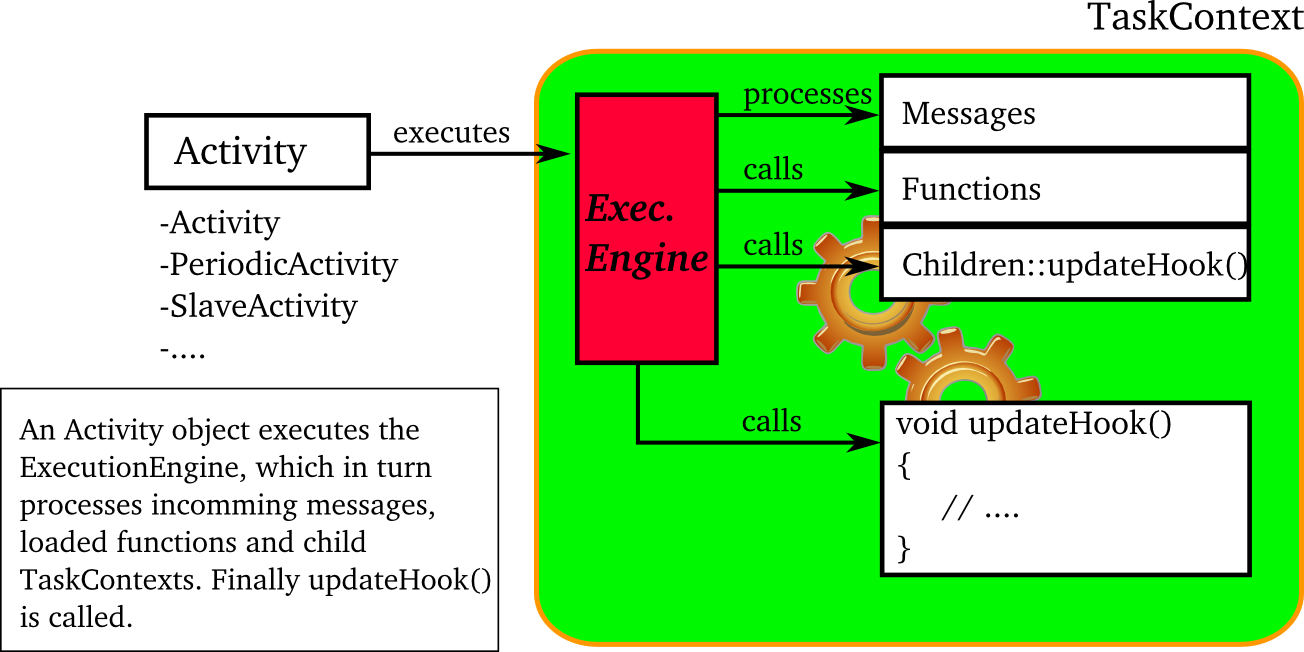
\includegraphics[width=.8\linewidth]{TaskContextExecution}
\end{center}
\end{frame}

\begin{frame}{Interconnexion des composants}{Flot de données}
\begin{itemize}
\item Connexion entre deux ports,
	\begin{itemize}
	\item Lock-free
	\end{itemize}
\item Politique de la connexion :
	\begin{itemize}
	\item donnée unique partagée (DATA) ou bufferisée (BUFFER)
	\item taille du buffer
	\item valeur initiale
	\end{itemize}
\item Chaque composant peut :
	\begin{itemize}
	\item Lire ou écrire dans son port,
	\item Connaitre l'état de la connexion,
	\item Savoir si la donnée \structure{reçue} est nouvelle.
	\end{itemize}
\end{itemize}
\end{frame}

\begin{frame}{Interconnexion des composants}{Flot de services}
\begin{itemize}
\item Connexion des opérations (services fournis) d'un composant aux méthodes (services requis) d'un autre,
\item Utilise le nom du service et la signature des fonctions,
\item Le code associé (la fonction C++) est exécuté :
	\begin{itemize}
	\item Dans la tâche du fournisseur (le fournisseur doit l'autoriser),
	\item Dans la tâche du demandeur (le demandeur doit l'autoriser),
	\item Dans une tâche de fond de la RTT (si personne ne veut l'exécuter).
	\end{itemize}
\item Le demandeur peut choisir d'attendre le retour de la fonction (bloquant) ou non.
\end{itemize}
\end{frame}

\subsection{Déploiement}
\begin{frame}{Déploiement}{Architecture}
\begin{center}
\begin{tikzpicture}
\useasboundingbox (-.8,-.5) rectangle (7.6,3.7);
%\draw (0,0) grid (6,5);
\draw[thick,->] (0,.1) -| +(1,0) |- (2.4,.8);
\draw[thick,->] (0,1.6) -| +(1,0) |- (2.4,1);
\draw[thick,->] (3.8,1) -- +(1,0);
\foreach \x/\y in {1.2/-2.1,2.5/-.3,-1.2/-2.1,-2.5/-.3,-4.3/-1.2} {
	\draw[thick,dashed,->] (4.3,3.1) -- ++(0,.5) -| ++(\x,\y);
}
\foreach \c/\x/\y in {Camera/0/0,Nav./0/1.8,Mapping/3.1/.9,Zoning/5.5/.9,%
	PathPl./1.8/2.7,MissionPl/6.8/2.7,Superv./4.3/2.7} {
	\node at (\x,\y) {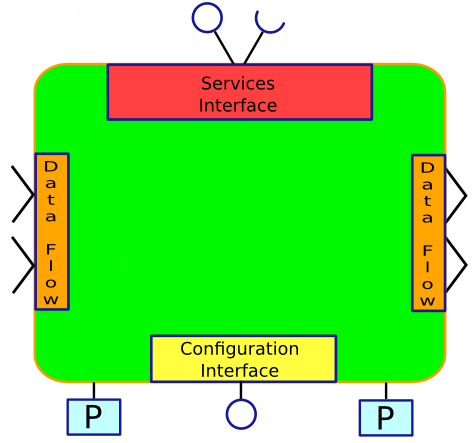
\includegraphics[width=.15\linewidth]{component}};\node at (\x,\y) {\tt \scriptsize \c};
}
\draw[thick,->] (4.5,-.3) -- +(.5,0); \node at (5.8,-.3) {\scriptsize data flow};
\draw[thick,dashed,->] (4.5,-.6) -- +(.5,0); \node at (5.8,-.6) {\scriptsize control flow};
\end{tikzpicture}
\end{center}
\end{frame}

\begin{frame}{OCL::DeploymentComponent}
\begin{center}
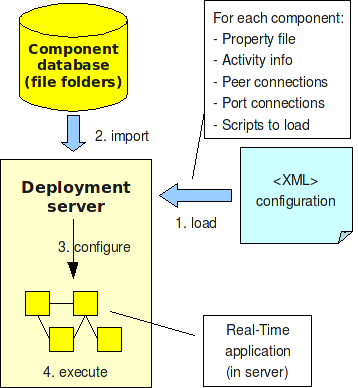
\includegraphics[width=.5\linewidth]{Deployment}
\end{center}
\end{frame}

\begin{frame}[containsverbatim]{Fichier XML}
\lstset{language=XML,basicstyle=\tiny,tabsize=1}
\begin{lstlisting}[frame=trBL]
<properties>
	<!-- Imports -->
	<simple name="Import" type="string">
		<value>libressac-mapping</value>
	</simple>
	...
	<!-- Components -->
	<struct name="Mapping" type="Ressac::Mapping">
		<struct name="Activity" type="Activity">
			<simple name="Period" type="double"><value>0</value></simple>
			<simple name="Priority" type="short"><value>0</value></simple>
			<simple name="Scheduler" type="string">
				<value>ORO_SCHED_OTHER</value></simple>
		</struct>
		<struct name="Properties" type="PropertyBag">
			<struct name="Matching" type="PropertyBag">
				<simple name="rSearch" type="short"><value>100</value></simple>
			</struct>
		</struct>
		<simple name="AutoConf" type="boolean"><value>1</value></simple>
		<simple name="AutoStart" type="boolean"><value>0</value></simple>
	</struct>
\end{lstlisting}
\end{frame}

\begin{frame}[containsverbatim]{Fichier XML}
\lstset{language=XML,basicstyle=\tiny,tabsize=1}
\begin{lstlisting}[frame=trBL]
	<struct name="Camera" type="RoboTIS::Vision::FirewireCamera"></struct>
	<struct name="Zoning" type="Ressac::Zoning"></struct>
	<struct name="Planning" type="Planning::PlannerHMDP"></struct>
	<struct name="Navigation" type="Ressac::NavigationOutSerial"></struct>
	<struct name="Ressac">
		<simple name="StateMachineScript" type="string">
			<value>search_and_rescue.osd</value>
		</simple>
	</struct>
\end{lstlisting}
\end{frame}

\subsection{Supervision}
\begin{frame}{Machine à états}
\begin{center}
\begin{tikzpicture}[
	scale=0.6,transform shape,
	node distance=25mm,
	statenode/.style={
		rectangle,minimum width=20mm,minimum height=10mm,rounded corners=3mm,
		text centered,very thick,draw=black!50,
		top color=white,bottom color=black!20,font=\ttfamily\small},
	entrynode/.style={circle,draw=black,fill=black},
	transition/.style={->,thick,draw=black!50},
	event/.style={
		rectangle,minimum size=6mm,text centered,
		dashed,thick,midway,font=\itshape\tiny}
	]
 	\node [statenode, minimum height=2.5cm, minimum width=6cm] (initGo) at (2.5,.5) {\begin{tabular}{l}
		InitialGo\\\hline\vspace{1.5cm}\end{tabular}};
	\node [statenode, minimum height=2.5cm, minimum width=6cm] (initExp) at (9.5,.5) {\begin{tabular}{l}
		InitialExplore\\\hline\vspace{1.5cm}\end{tabular}};
	\node [entrynode,left of=initGo, node distance=5cm] (entry) {};
 	\draw [transition] (entry) -- (initGo) node[event] {/ Nav.phase(HOVER)};
 	\draw [transition] (initGo) -- (initExp);
	% GOTO
	\begin{scope}
		\node [entrynode] (entry) at (0,0) {};
 		\node [statenode, right of=entry] (going) {Going};
		\node [entrynode, right of=going] (exit) {};
	 	\draw [transition] (entry) -- (going) node[event] {/ Nav.goto(A)};
		\draw [transition] (going) -- (exit) node[event] {$|X-A|<\varepsilon$};
	\end{scope}
 	% EXPLORE
	\begin{scope}
		\node [entrynode] (entry) at (7,0) {};
 		\node [statenode, right of=entry] (going) {Exploring};
		\node [entrynode, right of=going] (exit) {};
	 	\draw [transition] (entry) -- (going) node[event] {/ Nav.follow(p)};
		\draw [transition] (going) -- (exit) node[event] {X == p.last};
	\end{scope}
 	\node [statenode] (zoning) at (9.5,-4) {Zoning};
 	\node [statenode] (loadPb) at (6,-4) {LoadProblem};
 	\node [statenode] (execPol) at (2,-4) {ExecPolicy};
 	\node [statenode] (gotoBase) at (4,-6) {GotoBase};
 	\node [statenode] (goto) at (0,-6) {Goto};
 	\node [statenode] (explore) at (-2,-4) {Explore};
 	\node [statenode] (land) at (0,-2) {Land};
 	\node [statenode] (to) at (4,-2) {TakeOff};
 	\node [entrynode, below of=gotoBase] (exit) {};

 	\draw [transition] (initExp) -- (zoning);
 	\draw [transition] (zoning) -- (loadPb) node[event] {$zones \neq \emptyset$};
 	\draw [transition] (zoning) -- (gotoBase) node[event] {$zones == \emptyset$};
 	\draw [transition] (loadPb) -- (execPol);
 	\draw [transition] (gotoBase) -- (exit);
 	\path (execPol) edge[transition,bend left=10] node[event]{gotoBase} (gotoBase)
	 		edge[transition,bend left=10] node[event]{goto} (goto)
 			edge[transition,bend left=10] node[event]{explore} (explore)
 			edge[transition,bend left=10] node[event]{land} (land)
 			edge[transition,bend left=10] node[event]{takeOff} (to)
 		(gotoBase) edge[transition,bend left=10] (execPol)
 		(goto) edge[transition,bend left=10] (execPol)
 		(explore) edge[transition,bend left=10] (execPol)
 		(land) edge[transition,bend left=10] (execPol)
 		(to) edge[transition,bend left=10] (execPol);
\end{tikzpicture}
\end{center}
\end{frame}

\begin{frame}[containsverbatim]{Fichier OSD}
\lstset{language=C++,basicstyle=\tiny,tabsize=1}
\begin{lstlisting}[frame=trBL]
StateMachine SearchAndRescue {
	param zone z
	var zones zone_list

	initial state Init {
		transition select InitialGo
	}

	state InitialGo {
		entry {
			do Navigation.goto(z.center)
		}
		transition select InitialExplore
	}
	
	state Zoning {
		entry {
			do Zoning.extract()
			set zone_list = Zoning.zone_list.Get()
		}
		transition if zone_list.size != 0 then select LoadProblem
		transition if zone_list.size == 0 then select GotoBase
	}
	...
\end{lstlisting}
\end{frame}

\end{document}
